\subsection{Parallelization}

Parallelization is an approach to computational problem solving where the computation is divided into smaller 
subproblems and each sub-problem is computed simultaneously. The results of each sub-problem are then combined 
to get the final result of the whole computation.

The process of parallelizing a computation can be taken at different levels, from the bit level on a single machine 
to distributed computing over multiple machines (using cluster or grid computing).

\paragraph{Multiple Threading and Processes} Independent computation tasks may be delegated across separate processor cores by using threads or processes. When processing large cascades, we can make use of these techniques in order to reduce computation time.

\paragraph{Avoiding Global Interpreter Lock} When using an interpreted programming language such as Python, it is important to keep in mind that if each thread is running in the same interpreter instance, it is possible that one thread may ``lock'' the interpreter, preventing the execution of the other threads. Thus, rather than using threads, Revsim uses \emph{subprocesses} in order to delegate tasks to separate processor cores. Each subprocess runs its own interpreter instance, thus sidestepping Global Interpreter Lock. This advantage comes at the cost of increased interpreter overhead, but this cost is negligible when the benefits of subprocessing are considered. 

\paragraph{Parallelization in Revsim} 
In order to efficiently optimize large cascades on multi-processing systems, Revsim uses a ``splitting'' approach, wherein cascades are partitioned into sub-cascade ``blocks'', which are then optimized independently. Each block is passed through a corresponding instance of the GeneticAlgorithm class, which runs in a Python subprocess. The host operating system is then free to delegate the subprocess to a particular CPU or core, which allows This process is illustrated in Figure {\bf [REF!]}.
\begin{figure}
  \begin{center}
    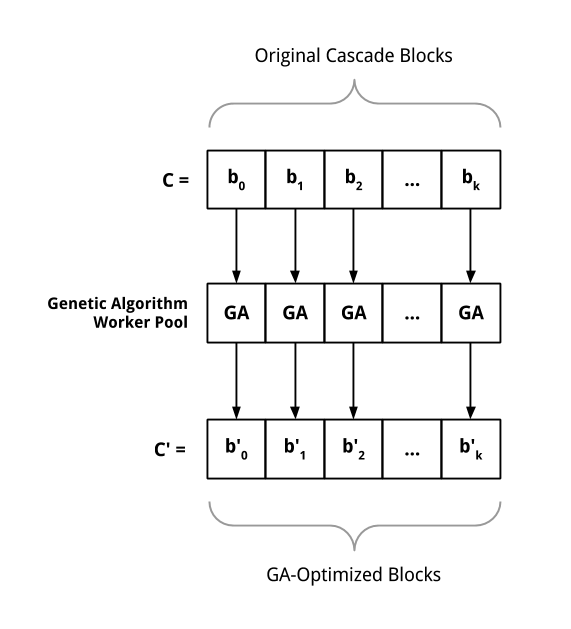
\includegraphics[width=80mm]{diagrams/parallelization.png}
  \end{center}
  \caption{Parallelization in Revsim.}
\end{figure}

Once a GeneticAlgorithm subprocess completes, the resulting (optimized) cascade is returned 


\paragraph{Grid Computing}
add basic definition: which is each node is generally loosely coupled, generally heterogeneous.